%% bare_jrnl.tex
%% V1.4b
%% 2015/08/26
%% by Michael Shell
%% see http://www.michaelshell.org/
%% for current contact information.
%%
%% This is a skeleton file demonstrating the use of IEEEtran.cls
%% (requires IEEEtran.cls version 1.8b or later) with an IEEE
%% journal paper.
%%
%% Support sites:
%% http://www.michaelshell.org/tex/ieeetran/
%% http://www.ctan.org/pkg/ieeetran
%% and
%% http://www.ieee.org/

%%*************************************************************************
%% Legal Notice:
%% This code is offered as-is without any warranty either expressed or
%% implied; without even the implied warranty of MERCHANTABILITY or
%% FITNESS FOR A PARTICULAR PURPOSE! 
%% User assumes all risk.
%% In no event shall the IEEE or any contributor to this code be liable for
%% any damages or losses, including, but not limited to, incidental,
%% consequential, or any other damages, resulting from the use or misuse
%% of any information contained here.
%%
%% All comments are the opinions of their respective authors and are not
%% necessarily endorsed by the IEEE.
%%
%% This work is distributed under the LaTeX Project Public License (LPPL)
%% ( http://www.latex-project.org/ ) version 1.3, and may be freely used,
%% distributed and modified. A copy of the LPPL, version 1.3, is included
%% in the base LaTeX documentation of all distributions of LaTeX released
%% 2003/12/01 or later.
%% Retain all contribution notices and credits.
%% ** Modified files should be clearly indicated as such, including  **
%% ** renaming them and changing author support contact information. **
%%*************************************************************************


% *** Authors should verify (and, if needed, correct) their LaTeX system  ***
% *** with the testflow diagnostic prior to trusting their LaTeX platform ***
% *** with production work. The IEEE's font choices and paper sizes can   ***
% *** trigger bugs that do not appear when using other class files.       ***                          ***
% The testflow support page is at:
% http://www.michaelshell.org/tex/testflow/



\documentclass[journal]{IEEEtran}
%
% If IEEEtran.cls has not been installed into the LaTeX system files,
% manually specify the path to it like:
% \documentclass[journal]{../sty/IEEEtran}





% Some very useful LaTeX packages include:
% (uncomment the ones you want to load)


% *** MISC UTILITY PACKAGES ***
%
%\usepackage{ifpdf}
\usepackage{graphicx}
% Heiko Oberdiek's ifpdf.sty is very useful if you need conditional
% compilation based on whether the output is pdf or dvi.
% usage:
% \ifpdf
%   % pdf code
% \else
%   % dvi code
% \fi
% The latest version of ifpdf.sty can be obtained from:
% http://www.ctan.org/pkg/ifpdf
% Also, note that IEEEtran.cls V1.7 and later provides a builtin
% \ifCLASSINFOpdf conditional that works the same way.
% When switching from latex to pdflatex and vice-versa, the compiler may
% have to be run twice to clear warning/error messages.






% *** CITATION PACKAGES ***
%
%\usepackage{cite}
% cite.sty was written by Donald Arseneau
% V1.6 and later of IEEEtran pre-defines the format of the cite.sty package
% \cite{} output to follow that of the IEEE. Loading the cite package will
% result in citation numbers being automatically sorted and properly
% "compressed/ranged". e.g., [1], [9], [2], [7], [5], [6] without using
% cite.sty will become [1], [2], [5]--[7], [9] using cite.sty. cite.sty's
% \cite will automatically add leading space, if needed. Use cite.sty's
% noadjust option (cite.sty V3.8 and later) if you want to turn this off
% such as if a citation ever needs to be enclosed in parenthesis.
% cite.sty is already installed on most LaTeX systems. Be sure and use
% version 5.0 (2009-03-20) and later if using hyperref.sty.
% The latest version can be obtained at:
% http://www.ctan.org/pkg/cite
% The documentation is contained in the cite.sty file itself.






% *** GRAPHICS RELATED PACKAGES ***
%
\ifCLASSINFOpdf
  % \usepackage[pdftex]{graphicx}
  % declare the path(s) where your graphic files are
  % \graphicspath{{../pdf/}{../jpeg/}}
  % and their extensions so you won't have to specify these with
  % every instance of \includegraphics
  % \DeclareGraphicsExtensions{.pdf,.jpeg,.png}
\else
  % or other class option (dvipsone, dvipdf, if not using dvips). graphicx
  % will default to the driver specified in the system graphics.cfg if no
  % driver is specified.
  % \usepackage[dvips]{graphicx}
  % declare the path(s) where your graphic files are
  % \graphicspath{{../eps/}}
  % and their extensions so you won't have to specify these with
  % every instance of \includegraphics
  % \DeclareGraphicsExtensions{.eps}
\fi
% graphicx was written by David Carlisle and Sebastian Rahtz. It is
% required if you want graphics, photos, etc. graphicx.sty is already
% installed on most LaTeX systems. The latest version and documentation
% can be obtained at: 
% http://www.ctan.org/pkg/graphicx
% Another good source of documentation is "Using Imported Graphics in
% LaTeX2e" by Keith Reckdahl which can be found at:
% http://www.ctan.org/pkg/epslatex
%
% latex, and pdflatex in dvi mode, support graphics in encapsulated
% postscript (.eps) format. pdflatex in pdf mode supports graphics
% in .pdf, .jpeg, .png and .mps (metapost) formats. Users should ensure
% that all non-photo figures use a vector format (.eps, .pdf, .mps) and
% not a bitmapped formats (.jpeg, .png). The IEEE frowns on bitmapped formats
% which can result in "jaggedy"/blurry rendering of lines and letters as
% well as large increases in file sizes.
%
% You can find documentation about the pdfTeX application at:
% http://www.tug.org/applications/pdftex





% *** MATH PACKAGES ***
%
%\usepackage{amsmath}
% A popular package from the American Mathematical Society that provides
% many useful and powerful commands for dealing with mathematics.
%
% Note that the amsmath package sets \interdisplaylinepenalty to 10000
% thus preventing page breaks from occurring within multiline equations. Use:
%\interdisplaylinepenalty=2500
% after loading amsmath to restore such page breaks as IEEEtran.cls normally
% does. amsmath.sty is already installed on most LaTeX systems. The latest
% version and documentation can be obtained at:
% http://www.ctan.org/pkg/amsmath





% *** SPECIALIZED LIST PACKAGES ***
%
%\usepackage{algorithmic}
% algorithmic.sty was written by Peter Williams and Rogerio Brito.
% This package provides an algorithmic environment fo describing algorithms.
% You can use the algorithmic environment in-text or within a figure
% environment to provide for a floating algorithm. Do NOT use the algorithm
% floating environment provided by algorithm.sty (by the same authors) or
% algorithm2e.sty (by Christophe Fiorio) as the IEEE does not use dedicated
% algorithm float types and packages that provide these will not provide
% correct IEEE style captions. The latest version and documentation of
% algorithmic.sty can be obtained at:
% http://www.ctan.org/pkg/algorithms
% Also of interest may be the (relatively newer and more customizable)
% algorithmicx.sty package by Szasz Janos:
% http://www.ctan.org/pkg/algorithmicx




% *** ALIGNMENT PACKAGES ***
%
%\usepackage{array}
% Frank Mittelbach's and David Carlisle's array.sty patches and improves
% the standard LaTeX2e array and tabular environments to provide better
% appearance and additional user controls. As the default LaTeX2e table
% generation code is lacking to the point of almost being broken with
% respect to the quality of the end results, all users are strongly
% advised to use an enhanced (at the very least that provided by array.sty)
% set of table tools. array.sty is already installed on most systems. The
% latest version and documentation can be obtained at:
% http://www.ctan.org/pkg/array


% IEEEtran contains the IEEEeqnarray family of commands that can be used to
% generate multiline equations as well as matrices, tables, etc., of high
% quality.




% *** SUBFIGURE PACKAGES ***
%\ifCLASSOPTIONcompsoc
%  \usepackage[caption=false,font=normalsize,labelfont=sf,textfont=sf]{subfig}
%\else
%  \usepackage[caption=false,font=footnotesize]{subfig}
%\fi
% subfig.sty, written by Steven Douglas Cochran, is the modern replacement
% for subfigure.sty, the latter of which is no longer maintained and is
% incompatible with some LaTeX packages including fixltx2e. However,
% subfig.sty requires and automatically loads Axel Sommerfeldt's caption.sty
% which will override IEEEtran.cls' handling of captions and this will result
% in non-IEEE style figure/table captions. To prevent this problem, be sure
% and invoke subfig.sty's "caption=false" package option (available since
% subfig.sty version 1.3, 2005/06/28) as this is will preserve IEEEtran.cls
% handling of captions.
% Note that the Computer Society format requires a larger sans serif font
% than the serif footnote size font used in traditional IEEE formatting
% and thus the need to invoke different subfig.sty package options depending
% on whether compsoc mode has been enabled.
%
% The latest version and documentation of subfig.sty can be obtained at:
% http://www.ctan.org/pkg/subfig




% *** FLOAT PACKAGES ***
%
%\usepackage{fixltx2e}
% fixltx2e, the successor to the earlier fix2col.sty, was written by
% Frank Mittelbach and David Carlisle. This package corrects a few problems
% in the LaTeX2e kernel, the most notable of which is that in current
% LaTeX2e releases, the ordering of single and double column floats is not
% guaranteed to be preserved. Thus, an unpatched LaTeX2e can allow a
% single column figure to be placed prior to an earlier double column
% figure.
% Be aware that LaTeX2e kernels dated 2015 and later have fixltx2e.sty's
% corrections already built into the system in which case a warning will
% be issued if an attempt is made to load fixltx2e.sty as it is no longer
% needed.
% The latest version and documentation can be found at:
% http://www.ctan.org/pkg/fixltx2e


%\usepackage{stfloats}
% stfloats.sty was written by Sigitas Tolusis. This package gives LaTeX2e
% the ability to do double column floats at the bottom of the page as well
% as the top. (e.g., "\begin{figure*}[!b]" is not normally possible in
% LaTeX2e). It also provides a command:
%\fnbelowfloat
% to enable the placement of footnotes below bottom floats (the standard
% LaTeX2e kernel puts them above bottom floats). This is an invasive package
% which rewrites many portions of the LaTeX2e float routines. It may not work
% with other packages that modify the LaTeX2e float routines. The latest
% version and documentation can be obtained at:
% http://www.ctan.org/pkg/stfloats
% Do not use the stfloats baselinefloat ability as the IEEE does not allow
% \baselineskip to stretch. Authors submitting work to the IEEE should note
% that the IEEE rarely uses double column equations and that authors should try
% to avoid such use. Do not be tempted to use the cuted.sty or midfloat.sty
% packages (also by Sigitas Tolusis) as the IEEE does not format its papers in
% such ways.
% Do not attempt to use stfloats with fixltx2e as they are incompatible.
% Instead, use Morten Hogholm'a dblfloatfix which combines the features
% of both fixltx2e and stfloats:
%
% \usepackage{dblfloatfix}
% The latest version can be found at:
% http://www.ctan.org/pkg/dblfloatfix




%\ifCLASSOPTIONcaptionsoff
%  \usepackage[nomarkers]{endfloat}
% \let\MYoriglatexcaption\caption
% \renewcommand{\caption}[2][\relax]{\MYoriglatexcaption[#2]{#2}}
%\fi
% endfloat.sty was written by James Darrell McCauley, Jeff Goldberg and 
% Axel Sommerfeldt. This package may be useful when used in conjunction with 
% IEEEtran.cls'  captionsoff option. Some IEEE journals/societies require that
% submissions have lists of figures/tables at the end of the paper and that
% figures/tables without any captions are placed on a page by themselves at
% the end of the document. If needed, the draftcls IEEEtran class option or
% \CLASSINPUTbaselinestretch interface can be used to increase the line
% spacing as well. Be sure and use the nomarkers option of endfloat to
% prevent endfloat from "marking" where the figures would have been placed
% in the text. The two hack lines of code above are a slight modification of
% that suggested by in the endfloat docs (section 8.4.1) to ensure that
% the full captions always appear in the list of figures/tables - even if
% the user used the short optional argument of \caption[]{}.
% IEEE papers do not typically make use of \caption[]'s optional argument,
% so this should not be an issue. A similar trick can be used to disable
% captions of packages such as subfig.sty that lack options to turn off
% the subcaptions:
% For subfig.sty:
% \let\MYorigsubfloat\subfloat
% \renewcommand{\subfloat}[2][\relax]{\MYorigsubfloat[]{#2}}
% However, the above trick will not work if both optional arguments of
% the \subfloat command are used. Furthermore, there needs to be a
% description of each subfigure *somewhere* and endfloat does not add
% subfigure captions to its list of figures. Thus, the best approach is to
% avoid the use of subfigure captions (many IEEE journals avoid them anyway)
% and instead reference/explain all the subfigures within the main caption.
% The latest version of endfloat.sty and its documentation can obtained at:
% http://www.ctan.org/pkg/endfloat
%
% The IEEEtran \ifCLASSOPTIONcaptionsoff conditional can also be used
% later in the document, say, to conditionally put the References on a 
% page by themselves.




% *** PDF, URL AND HYPERLINK PACKAGES ***
%
%\usepackage{url}
% url.sty was written by Donald Arseneau. It provides better support for
% handling and breaking URLs. url.sty is already installed on most LaTeX
% systems. The latest version and documentation can be obtained at:
% http://www.ctan.org/pkg/url
% Basically, \url{my_url_here}.




% *** Do not adjust lengths that control margins, column widths, etc. ***
% *** Do not use packages that alter fonts (such as pslatex).         ***
% There should be no need to do such things with IEEEtran.cls V1.6 and later.
% (Unless specifically asked to do so by the journal or conference you plan
% to submit to, of course. )


% correct bad hyphenation here
\hyphenation{op-tical net-works semi-conduc-tor}


\begin{document}
%
% paper title
% Titles are generally capitalized except for words such as a, an, and, as,
% at, but, by, for, in, nor, of, on, or, the, to and up, which are usually
% not capitalized unless they are the first or last word of the title.
% Linebreaks \\ can be used within to get better formatting as desired.
% Do not put math or special symbols in the title.
\title{Anomaly Identification in Big Data using Apache Spark }
%
%
% author names and IEEE memberships
% note positions of commas and nonbreaking spaces ( ~ ) LaTeX will not break
% a structure at a ~ so this keeps an author's name from being broken across
% two lines.
% use \thanks{} to gain access to the first footnote area
% a separate \thanks must be used for each paragraph as LaTeX2e's \thanks
% was not built to handle multiple paragraphs
%

% \author{Michael~Shell,~\IEEEmembership{Member,~IEEE,}
%         John~Doe,~\IEEEmembership{Fellow,~OSA,}
%         and~Jane~Doe,~\IEEEmembership{Life~Fellow,~IEEE}% <-this % stops a space
% \thanks{M. Shell was with the Department
% of Electrical and Computer Engineering, Georgia Institute of Technology, Atlanta,
% GA, 30332 USA e-mail: (see http://www.michaelshell.org/contact.html).}% <-this % stops a space
% \thanks{J. Doe and J. Doe are with Anonymous University.}% <-this % stops a space
% \thanks{Manuscript received April 19, 2005; revised August 26, 2015.}}

% note the % following the last \IEEEmembership and also \thanks - 
% these prevent an unwanted space from occurring between the last author name
% and the end of the author line. i.e., if you had this:
% 
% \author{....lastname \thanks{...} \thanks{...} }
%                     ^------------^------------^----Do not want these spaces!
%
% a space would be appended to the last name and could cause every name on that
% line to be shifted left slightly. This is one of those "LaTeX things". For
% instance, "\textbf{A} \textbf{B}" will typeset as "A B" not "AB". To get
% "AB" then you have to do: "\textbf{A}\textbf{B}"
% \thanks is no different in this regard, so shield the last } of each \thanks
% that ends a line with a % and do not let a space in before the next \thanks.
% Spaces after \IEEEmembership other than the last one are OK (and needed) as
% you are supposed to have spaces between the names. For what it is worth,
% this is a minor point as most people would not even notice if the said evil
% space somehow managed to creep in.



% The paper headers
% \markboth{Journal of \LaTeX\ Class Files,~Vol.~14, No.~8, August~2015}%
% {Shell \MakeLowercase{\textit{et al.}}: Bare Demo of IEEEtran.cls for IEEE Journals}
% The only time the second header will appear is for the odd numbered pages
% after the title page when using the twoside option.
% 
% *** Note that you probably will NOT want to include the author's ***
% *** name in the headers of peer review papers.                   ***
% You can use \ifCLASSOPTIONpeerreview for conditional compilation here if
% you desire.




% If you want to put a publisher's ID mark on the page you can do it like
% this:
%\IEEEpubid{0000--0000/00\$00.00~\copyright~2015 IEEE}
% Remember, if you use this you must call \IEEEpubidadjcol in the second
% column for its text to clear the IEEEpubid mark.



% use for special paper notices
%\IEEEspecialpapernotice{(Invited Paper)}




% make the title area
\maketitle

% As a general rule, do not put math, special symbols or citations
% in the abstract or keywords.
\begin{abstract}
In today's rapidly advancing digital landscape, where data growth surpasses historical benchmarks, innovative structures are required for efficient information retrieval from vast Big Data repositories. The Hadoop ecosystem, including HDFS, MapReduce, Hive, HBase, Pig, among others, addresses these complexities. Acknowledging the constraints of MapReduce, Apache Spark emerges as a pivotal player, processing data up to 100 times faster on memory. This transformative capability establishes Apache Spark as a key solution in the domain of Big Data processing, offering unmatched efficiency and scalability. Amid global concerns of credit card fraud, particularly in Bharat's (India's) expanding digital landscape, this paper explores sophisticated anomaly detection techniques, focusing on ~Isolation Forest and One-Class SVM algorithms. Practical considerations influence the choice to implement both, ensuring a balance between effectiveness and computational demands. The analysis evaluates their performance, providing insights into their suitability for credit card fraud detection within the constraints of the dataset and available computational power. Additionally, the research culminates in a nuanced exploration of the results, shedding light on the strengths and limitations of the ~Isolation Forest and One-Class SVM algorithms, as detailed in the concluding section.
\end{abstract}

% Note that keywords are not normally used for peerreview papers.
\begin{IEEEkeywords}
Big Data, Apache Spark, ~Isolation Forest, One-Class SVM, credit card, fraud detection.
\end{IEEEkeywords}






% For peer review papers, you can put extra information on the cover
% page as needed:
% \ifCLASSOPTIONpeerreview
% \begin{center} \bfseries EDICS Category: 3-BBND \end{center}
% \fi
%
% For peerreview papers, this IEEEtran command inserts a page break and
% creates the second title. It will be ignored for other modes.
\IEEEpeerreviewmaketitle



\section{Introduction}
% The very first letter is a 2 line initial drop letter followed
% by the rest of the first word in caps.
% 
% form to use if the first word consists of a single letter:
% \IEEEPARstart{A}{demo} file is ....
% 
% form to use if you need the single drop letter followed by
% normal text (unknown if ever used by the IEEE):
% \IEEEPARstart{A}{}demo file is ....
% 
% Some journals put the first two words in caps:
% \IEEEPARstart{T}{his demo} file is ....
% 
% Here we have the typical use of a "T" for an initial drop letter
% and "HIS" in caps to complete the first word.
\IEEEPARstart{I}{n} the contemporary era of rapid digital evolution, the monumental surge in data growth has surpassed historical benchmarks, fundamentally reshaping information management dynamics. Eric Schmidt's notable observation emphasizes that the volume of data generated from the inception of civilization until 2003 is now replicated in a mere two days, underscoring the unprecedented pace of data expansion. This exponential rise in data creation, exemplified by Twitter processing 340 million messages weekly and Facebook users generating 2.7 billion comments and likes, has propelled us into an era where the last year alone witnessed data generation equivalent to the cumulative output of the past 15 years.

This surge, measured in Exa and Zeta bytes, transcends traditional Tera and Peta byte metrics, necessitating innovative structures and intelligent processing capabilities for swift information retrieval from Big Data repositories within research institutes and enterprises. The widely embraced Hadoop ecosystem, encompassing HDFS, MapReduce, Hive, HBase, Pig, among others, has emerged as a robust solution to navigate and harness the complexities associated with such colossal data sets.

Big Data, characterized by high speed, volume, and variety, demands sophisticated frameworks for efficient decision-making and insight generation. MapReduce, introduced by Google in 2004 and implemented in the open-source Hadoop system, has played a pivotal role in diverse data analytics use cases, including reporting, OLAP, web data search, machine learning, data mining, and social networking analysis. Acknowledging the constraints of MapReduce, Apache Spark has emerged as its advanced counterpart, processing data up to 100 times faster than MapReduce on memory by minimizing read/write operations to disk and storing intermediate data in memory. This transformative capability establishes Apache Spark as a pivotal player in the domain of Big Data processing, offering unparalleled efficiency and scalability.

Credit card fraud remains a persistent and evolving concern that poses a significant threat to financial institutions and cardholders worldwide. The surge in digital transactions has created new opportunities for fraudsters to exploit vulnerabilities, resulting in substantial financial losses and eroding trust among stakeholders. Addressing this challenge necessitates the development of robust fraud detection systems capable of adapting to the dynamic nature of fraudulent activities.

In the context of Bharat, a rapidly growing economy characterized by an expanding digital landscape, the relevance of advanced anomaly detection techniques, particularly in credit card fraud detection, has never been more pronounced. The escalating adoption of digital payments, driven by government initiatives and increased smartphone penetration, amplifies the risk of fraudulent activities. The exploration of effective fraud detection methods in this paper holds the potential to safeguard financial interests, strengthen security measures, and foster a secure digital ecosystem in the Indian context.

Moreover, the escalating number of fraud incidents in Bharat underscores the urgency of implementing advanced detection measures. Year after year, the instances of fraud are on the rise, reflecting the pressing need for innovative and adaptive strategies to counteract this trend. The following [Fig. \ref{fig:yearly data}] graphical representation visually depicts the increasing number of fraud cases annually, emphasizing the imperative for proactive and effective countermeasures in the Indian credit card landscape.

\begin{figure}
    \centering
    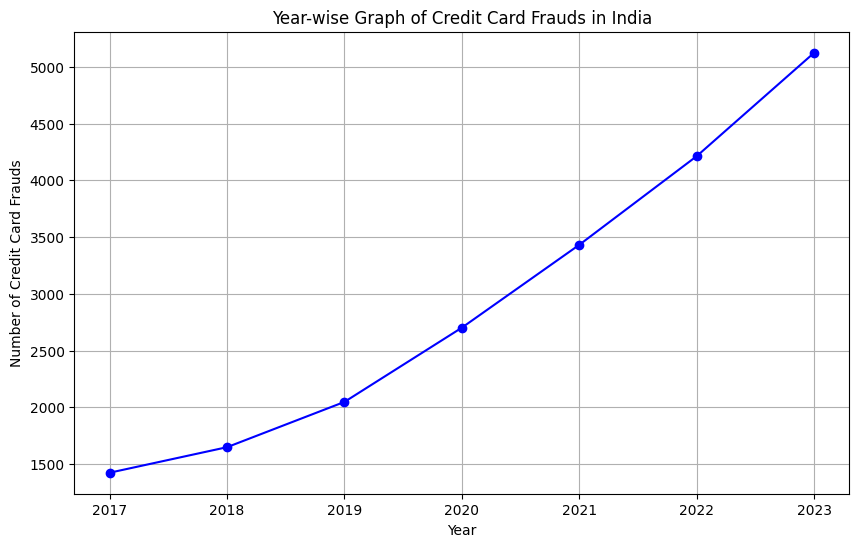
\includegraphics[width=0.9 \linewidth]{graph.png}
    \caption{Year Wise Credit Card Frauds in  \cite{livemint_card_frauds}}
    \label{fig:yearly data}
\end{figure}

We employ sophisticated anomaly detection techniques to address the formidable challenge of detecting anomalies in a highly imbalanced dataset. This paper primarily focuses on two algorithms: ~Isolation Forest\cite{isolationForest} and One-Class SVM\cite{One-classSVM}. Leveraging the power of isolation forests, we aim to efficiently isolate anomalies, making it particularly effective in fraud detection. Its simplicity and effectiveness in dealing with imbalanced datasets make it an attractive choice. The One-Class Support Vector Machine, designed for imbalanced classification tasks, offers another robust solution for anomaly detection. Its straightforward implementation and effectiveness in identifying anomalies make it a valuable addition to our methodology.

Practical considerations influence our choice to implement both algorithms. Given our computational constraints, executing complex algorithms can be resource-intensive. By implementing these two approaches, we balance effectiveness and computational demands. This approach allows us to explore the nuances and trade-offs between the algorithms while ensuring that the implementation remains feasible within the confines of our computational resources.
    
    In our analysis, we will evaluate the performance of both ~Isolation Forest and One-Class SVM, examining the differences in their outputs and providing insights into their suitability for credit card fraud detection in the context of our dataset and available computational power.

 
% You must have at least 2 lines in the paragraph with the drop letter
% % (should never be an issue)
% I wish you the best of success.

% \hfill mds
 
% \hfill August 26, 2015

% \subsection{Subsection Heading Here}
% Subsection text here.

% needed in second column of first page if using \IEEEpubid
%\IEEEpubidadjcol

% \subsubsection{Subsubsection Heading Here}
% Subsubsection text here.


% An example of a floating figure using the graphicx package.
% Note that \label must occur AFTER (or within) \caption.
% For figures, \caption should occur after the \includegraphics.
% Note that IEEEtran v1.7 and later has special internal code that
% is designed to preserve the operation of \label within \caption
% even when the captionsoff option is in effect. However, because
% of issues like this, it may be the safest practice to put all your
% \label just after \caption rather than within \caption{}.
%
% Reminder: the "draftcls" or "draftclsnofoot", not "draft", class
% option should be used if it is desired that the figures are to be
% displayed while in draft mode.
%
%\begin{figure}[!t]
%\centering
%\includegraphics[width=2.5in]{myfigure}
% where an .eps filename suffix will be assumed under latex, 
% and a .pdf suffix will be assumed for pdflatex; or what has been declared
% via \DeclareGraphicsExtensions.
%\caption{Simulation results for the network.}
%\label{fig_sim}
%\end{figure}

% Note that the IEEE typically puts floats only at the top, even when this
% results in a large percentage of a column being occupied by floats.


% An example of a double column floating figure using two subfigures.
% (The subfig.sty package must be loaded for this to work.)
% The subfigure \label commands are set within each subfloat command,
% and the \label for the overall figure must come after \caption.
% \hfil is used as a separator to get equal spacing.
% Watch out that the combined width of all the subfigures on a 
% line do not exceed the text width or a line break will occur.
%
%\begin{figure*}[!t]
%\centering
%\subfloat[Case I]{\includegraphics[width=2.5in]{box}%
%\label{fig_first_case}}
%\hfil
%\subfloat[Case II]{\includegraphics[width=2.5in]{box}%
%\label{fig_second_case}}
%\caption{Simulation results for the network.}
%\label{fig_sim}
%\end{figure*}
%
% Note that often IEEE papers with subfigures do not employ subfigure
% captions (using the optional argument to \subfloat[]), but instead will
% reference/describe all of them (a), (b), etc., within the main caption.
% Be aware that for subfig.sty to generate the (a), (b), etc., subfigure
% labels, the optional argument to \subfloat must be present. If a
% subcaption is not desired, just leave its contents blank,
% e.g., \subfloat[].


% An example of a floating table. Note that, for IEEE style tables, the
% \caption command should come BEFORE the table and, given that table
% captions serve much like titles, are usually capitalized except for words
% such as a, an, and, as, at, but, by, for, in, nor, of, on, or, the, to
% and up, which are usually not capitalized unless they are the first or
% last word of the caption. Table text will default to \footnotesize as
% the IEEE normally uses this smaller font for tables.
% The \label must come after \caption as always.
%
%\begin{table}[!t]
%% increase table row spacing, adjust to taste
%\renewcommand{\arraystretch}{1.3}
% if using array.sty, it might be a good idea to tweak the value of
% \extrarowheight as needed to properly center the text within the cells
%\caption{An Example of a Table}
%\label{table_example}
%\centering
%% Some packages, such as MDW tools, offer better commands for making tables
%% than the plain LaTeX2e tabular which is used here.
%\begin{tabular}{|c||c|}
%\hline
%One & Two\\
%\hline
%Three & Four\\
%\hline
%\end{tabular}
%\end{table}


% Note that the IEEE does not put floats in the very first column
% - or typically anywhere on the first page for that matter. Also,
% in-text middle ("here") positioning is typically not used, but it
% is allowed and encouraged for Computer Society conferences (but
% not Computer Society journals). Most IEEE journals/conferences use
% top floats exclusively. 
% Note that, LaTeX2e, unlike IEEE journals/conferences, places
% footnotes above bottom floats. This can be corrected via the
% \fnbelowfloat command of the stfloats package.


% \begin{table*}[hb]
% \begin{center}
% \begin{tabular}{|c|c|c|c|}
%   \hline
%   Reference Paper& Author Name & Objectives & Limitations \\ 
%   \hline
%   [1]& H. Ahmed and M. A. Ismail &  4 & 5 \\ 
%   \hline
%   [2]& J.M. Johnson and T.M. Khoshgoftaar  & 4 & 5 \\ 
%   \hline
%   [3]& Marcos R. Machado and Salma Karray & 4 & 5 \\ 
%   \hline
%   [4]& M. Bansal, I. Chana and S. Clarke    & The paper  & This \\ 
%   \hline
%   [5]& S. D. Khudhur and H. A. Jeihad  & The paper & The paper  \\ 
%   \hline
%   [6]& E. Kafeza, A. Kanavos, P. Vikatos, and S. Sioutas & The paper  &  The \\ 
%   \hline
% \end{tabular}
% \caption{Your caption here.}
% \end{center}
% \end{table*}

\section{Related Work}

Anomaly detection, particularly in credit card fraud, has become a central focus for researchers and data scientists. This section offers a concise overview of the existing literature, highlighting key research efforts that form the basis for our investigation into anomaly identification in credit card transactions.

One noteworthy contribution in the realm of big data identification is the structured approach proposed by Hameeza Ahmed et al. \cite{3V}, leveraging the 3Vs characteristics (Volume, Velocity, and Variety). Our proposed approach shares similarities with this work but advances further by quantifying and representing big data mathematically, incorporating application, data, and platform characteristics. This enhancement facilitates a nuanced understanding of big data, enabling the prescription of optimal resources for dynamic big data applications in a static context.

Addressing class label noise in big data classification is a critical challenge, as highlighted by J.M. Johnson et al. \cite{LNoise}. Their comprehensive survey categorizes label noise identifiers into three groups: distance-based techniques, ensemble techniques, and single-learner techniques. Moreover, they discuss strategies for treating label noise, including ignoring, removing, and correcting it. The review covers 30 methods, encompassing distributed solutions, deep learning techniques, and streaming techniques, providing valuable insights into mitigating class label noise in big data contexts.

In the dynamic landscape of big data analytics, researchers have made significant strides in diverse domains. M. Bansal et al. \cite{iot} delve into the Internet of Things in Big Data (IoTBD), offering a comprehensive exploration of key technologies, applications, and unique challenges associated with IoTBD, emphasizing its potential to revolutionize various industries. Another notable contribution comes from the lightweight machine learning-based approach, LSDStrategy, addressing the big data variety in multimedia streaming \cite{LSD}. LSDStrategy distinguishes itself by its easy implementation on edge devices, absence of the need for labeled data for the minority class, and an evaluating voting technique optimizing the classifier for accuracy and prediction time trade-offs. Additionally, E. Kafeza et al.'s work on "Twitter Personality-based Communicative Communities Extraction System for Big Data" introduces T-PCCE, a system that focuses on extracting communicative communities from Twitter based on user personality \cite{twitter}. This unique approach considers user personality, recognizing its significant role in shaping interactions and community formations on social media platforms. 

The paper "A Technological Survey on Apache Spark and Hadoop Technologies" by Dr. Nadeem et al. \cite{spark}offers a comprehensive overview of Apache Spark and its distinctive features, emphasizing its in-memory processing capabilities and versatile language support. The subsequent comparative study between Apache Spark and Hadoop reveals that Apache Spark excels in specific tasks, particularly iterative algorithms and machine learning applications. However, the paper acknowledges that Hadoop remains a robust choice for tasks demanding high throughput and scalability.

The following paper, "Big Data Analytics Techniques for Credit Card Fraud Detection" by M. Sathyapriya et al. \cite{CreditCard} continues to support the findings in the paper above \cite{spark} by offering a thorough review of big data analytics techniques for credit card fraud detection. Addressing challenges in big data, which include volume, velocity, veracity and data variety, the authors emphasize the necessity for scalable and efficient tools and algorithms. Their review encompasses various big data analytics techniques, leveraging Apache Hadoop, MapReduce, Apache Spark, and Apache Flink for credit card fraud detection. 


This paper tries to take advantage of the efficiency and speed that Apache Spark provides over other big data tools and evaluate the isolation forest algorithm in providing a quick and better result in credit card fraud detection.
\begin{table*}[btp]
\caption{Related works Comparative study}
    \centering
    \begin{tabular}{|c|p{1.7cm}|p{3.4cm}|p{2.2cm}|p{2.2cm}|p{2.2cm}|p{2.2cm}|}
        \hline
        \textbf{Reference} & \textbf{Author Name} & \textbf{Objectives} & \textbf{Evaluation} & \textbf{Result} & \textbf{Observation} & \textbf{Limitations} \\
        \hline
        1 & Johnson, Justin M. and Khoshgoftaar, Taghi M & Summarize challenges and techniques for classifying big data with label noise. & Categorized methods into three groups: distance-based, ensemble, single learner. & Label noise degrades machine learning performance, but various methods can mitigate it. & Label noise is pervasive, methods vary in effectiveness, more research is needed. & Focus on class label noise, classification tasks, English studies. \\
        \hline
        2 & Naghib, Arezou, Jafari Navimipour, Nima, Hosseinzadeh, Mehdi, Sharifi, Arash & Summarize BDM techniques, frameworks, and quality attributes in IoT. & Categorized BDM techniques into four groups. & Wide range of BDM techniques, choice depends on application requirements. & Quality attributes crucial for IoT BDM, open challenges exist. & Focus on BDM techniques, limited to English studies, no comprehensive evaluation. \\
        \hline
        3 & Kolajo, Taiwo, Daramola, Olawande, Adebiyi, Ayodele & Provide an overview of big data stream analysis (BDSA) techniques and challenges. & Conducted a systematic literature review to gather and analyze relevant studies. & BDSA techniques encompass data mining, stream processing, and machine learning approaches. & Real-time analysis and fault tolerance are crucial considerations for BDSA systems. & Does not provide a comprehensive evaluation of the effectiveness of different BDSA techniques. \\
        \hline
        4 & Kafeza, Eleanna, Kanavos, Andreas, Makris, Christos, Pispirigos, Georgios, Vikatos, Pantelis & Identify communicative communities in Twitter using personality-based approach. & Proposed T-PCCE system, evaluated using real-world Twitter data. & T-PCCE effectively identifies communicative communities based on user personality. & Personality plays a significant role in shaping communication patterns. & Focus on Twitter data, may not generalize to other social media platforms. \\
        \hline
        5 & Ahmed, Nadeem, Afthab, Asif, Nezami, Mohammed Mazhar & Compare and contrast Apache Spark and Hadoop. & Conducted literature review, analyzed performance metrics. & Spark outperforms Hadoop in many scenarios, but Hadoop still relevant for certain tasks. & Apache Spark and Hadoop are complementary technologies. & Focus on technical aspects, not specific applications. \\
        \hline
        6 & Sathyapriya, M., Thiagarasu, V. & Review big data analytics techniques for credit card fraud detection. & Comprehensive review of literature, evaluation of techniques. & Various big data analytics techniques can effectively detect credit card fraud. & Big data analytics offers promising solutions for credit card fraud detection. & Focus on technical aspects, not specific implementation details. \\
        \hline
    \end{tabular}
    
\end{table*}
\section{Methodology}
Credit card frauds are identified by using several input factors: time, amount and other factors which have undergone PCA transformation. [Fig. \ref{fig:flowchart}] represents the approach and flow by which Apache Spark, with the help of multiple algorithms, is used to detect fraud in the given dataset.

Our research relies on an open-source dataset of credit card transactions from September 2013, encompassing two days and totaling 284,807 instances, with only 492 classified as frauds (0.172\% of all transactions). Reflecting the real-world rarity of credit card fraud, this dataset presents a severe class imbalance. All features, except 'Time' and 'Amount,' undergo Principal Component Analysis (PCA) transformation, with V1 through V28 representing the principal components. Due to confidentiality, the original features remain undisclosed. 'Time' signifies seconds elapsed since the first transaction, 'Amount' denotes transaction value, and the 'Class' variable indicates fraud (1) or legitimate (0) transactions.


\begin{figure}[h]
  \centering
  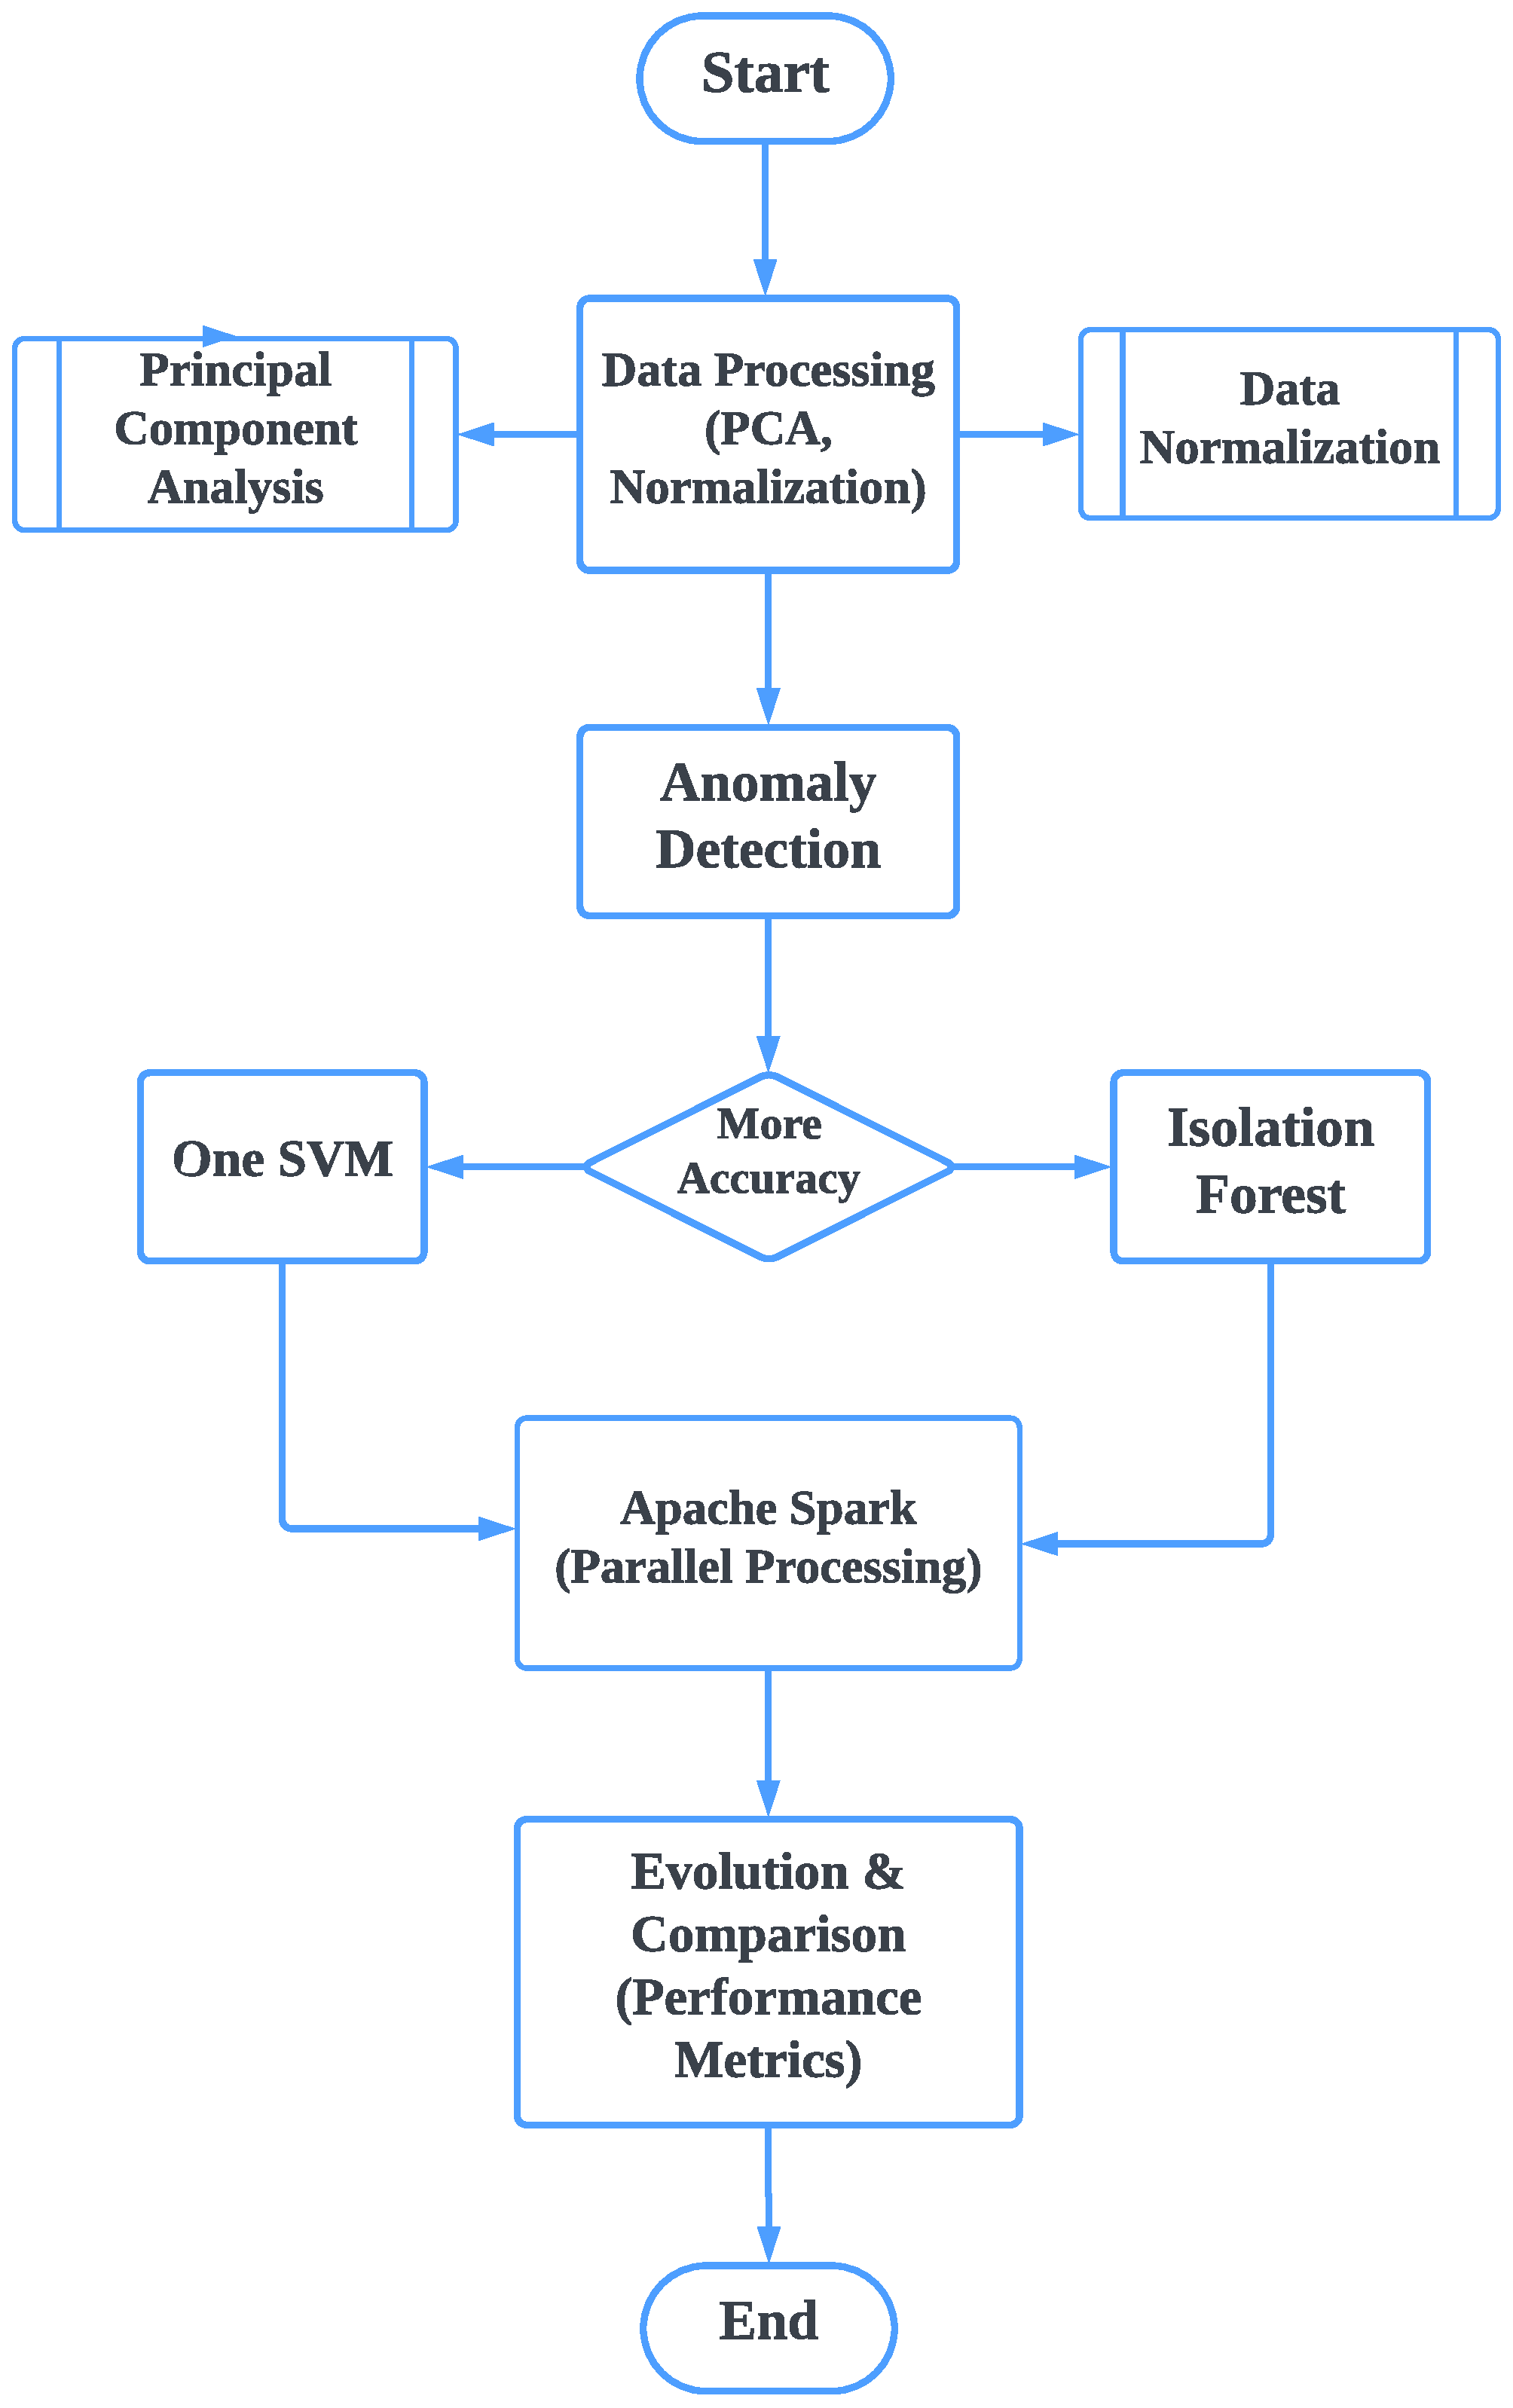
\includegraphics[width=0.7\linewidth]{vertical.eps}
  \caption{Procedure to detect credit card fraud}
  \label{fig:flowchart}
\end{figure}


\textbf{Dataset Preprocessing:} 
In the context of credit card fraud detection, preparing the dataset for efficient analysis is vital. We apply Principal Component Analysis (PCA) to address the challenges posed by high-dimensional data, a common feature in credit card transaction records. PCA transforms the data matrix X into a lower-dimensional space X pca by multiplying it with the matrix of principal components W, represented as:  \(X_pca = X * W\)

PCA reduces the dimensionality of the dataset while retaining essential information. This reduces the risk of overfitting by eliminating noise and enhances computational efficiency. All features, except 'Time' and 'Amount,' undergo PCA transformation, providing a balanced approach to data dimensionality.
As customary in financial data research, the original features and background information remain undisclosed for confidentiality reasons. 

\textbf{Data Normalization:} Data normalization is applied to ensure that all features are on a common scale, preventing any single attribute from unduly influencing the anomaly detection process. These preprocessing steps optimize the dataset for subsequent analysis with the ~Isolation Forest and One-Class SVM algorithms, and they facilitate efficient utilization of Apache Spark for distributed processing, which is a central aspect of our research methodology.

To detect anomalies in credit card transactions, we deploy two carefully selected algorithms: Isolation Forest and One-Class SVM. These choices are made with precision to address the specific challenges posed by our dataset and the inherent nature of credit card fraud detection.

\textbf{Isolation Forest:} A potent anomaly detection algorithm, excels in isolating anomalies within datasets, especially those with imbalanced class distributions. Given the severe class imbalance in our dataset, where only a minute fraction of transactions are categorized as fraud (0.172 percent), ~Isolation Forest's ability to efficiently isolate anomalies is crucial. We opt for Isolation Forest due to its simplicity and effectiveness in handling imbalanced datasets. Its innate capacity to isolate anomalies without complex feature engineering makes it an appealing choice for our research.

\textbf{One-Class SVM:} A robust algorithm tailored for imbalanced classification tasks, offers a straightforward implementation and is renowned for its effectiveness in identifying anomalies. The deliberate selection of ~Isolation Forest and One-Class SVM is informed by practical considerations. While more complex algorithms may yield optimal results, their computational demands can be resource-intensive. By implementing these two complementary approaches, we strike a balance between efficacy and computational feasibility. This strategy enables us to explore the nuances and trade-offs between the two algorithms, ensuring our implementation remains within the confines of available computational resources.

Furthermore, concurrently implementing both algorithms is expected to yield superior accuracy. This multi-algorithm approach will be thoroughly evaluated in our analysis, affording a comprehensive understanding of their suitability in credit card fraud detection within the context of our dataset and computational infrastructure.

\textbf{Parallel Processing with Apache Spark:} In our endeavor to achieve effective anomaly detection in credit card transactions, the pivotal role of Apache Spark in distributed data processing cannot be overstated. Apache Spark, a versatile and powerful framework, forms the cornerstone of our research methodology, providing a robust foundation for large-scale data analysis.

Advantages of Apache Spark- The utilization of Apache Spark is underpinned by its inherent advantages, strategically aligned with the demands of our research. These advantages play a crucial role in the success of our project:
Speed and Efficiency: The speed and computational efficiency facilitated by Apache Spark's in-memory processing are paramount. Real-time anomaly detection is significantly accelerated, enabling the swift identification of fraudulent transactions.
Scalability: The innate scalability of Apache Spark, allowing for horizontal expansion, positions it as the ideal platform for managing the voluminous datasets characteristic of credit card transactions. This scalability effortlessly accommodates the extensive data volume at the heart of our research.
Ease of Use: Apache Spark's user-friendly APIs and compatibility with various programming languages enhance the efficiency of implementing complex algorithms. This streamlined approach contributes to the overall success of our project.
Apache Spark's intrinsic capabilities are seamlessly integrated into our research objectives, making it a fundamental contributor to our project:
Efficient Data Processing: The parallel processing capabilities of Apache Spark empower our research to manage the dataset's scale and complexity without sacrificing performance. This ensures timely and effective fraud detection.
\newline
Resource Optimization: Apache Spark's ability to optimize resource usage ensures that the available computational power is effectively harnessed, aligning perfectly with our multi-algorithm approach.
\newline
Real-Time Processing: The exceptional speed and efficiency of Apache Spark enable real-time anomaly detection, enhancing our ability to respond promptly to potentially fraudulent activities.
\newline
Scalable Framework: Apache Spark's inherent scalability ensures our methodology remains adaptable and resilient to the evolving landscape of credit card transactions, effectively addressing new challenges and accommodating increasing data volumes.

In conclusion, Apache Spark serves as the bedrock of our research methodology, furnishing the essential distributed data processing capabilities required to analyze extensive credit card transaction data efficiently. Its advantages, encompassing speed, scalability, and resource optimization, harmoniously align with our research objectives and substantially enhance our ability to identify and combat fraud effectively.


\textbf{Evaluation and Comparison:} In this phase, our primary objective is to assess the performance of the ~Isolation Forest and One-Class SVM algorithms in the context of credit card fraud detection, which is the focal point of our research.

We have carefully selected key evluation metrics tailored to our imbalanced dataset and the unique challenges of fraud detection:
\newline
1. AUPRC\cite{AUPRC} (Area Under the Precision-Recall Curve): This metric is particularly suited to our project, considering its focus on imbalanced datasets. It offers insights into precision and recall, essential in effectively identifying fraud.

2. F1-Score: We utilize the F1-score to strike a balance between precision and recall, aligning it with our project's objective of finding the best trade-off between these two metrics.

3. ROC Curve and AUC-ROC: While AUC-ROC is a common metric, we are mindful of its limitations on highly imbalanced datasets. However, it still provides valuable insights into the model's discriminatory power.

4. Confusion Matrix: This matrix helps us understand the model's performance intricacies, including false positives and negatives, which are paramount in credit card fraud detection.

Our evaluation aims to offer clear insights into the suitability of the ~Isolation Forest and One-Class SVM algorithms for our specific project, addressing the challenges inherent in credit card fraud detection within the context of our dataset.

\section{Experimental Results}

\subsection{Experimental Setup}
The experimental setup incorporated the use of PySpark, a powerful open-source distributed computing framework, to construct and streamline machine learning pipelines. Leveraging PySpark's capabilities, we designed and executed end-to-end pipelines encompassing data preprocessing, feature engineering, and model training. PySpark's distributed computing paradigm allowed for the efficient handling of large-scale datasets, a critical aspect in credit card fraud detection where the dataset often involves a substantial number of transactions. The PySpark MLlib library facilitated the implementation of machine learning algorithms within the Spark framework, ensuring scalability and parallel processing.

Within the PySpark pipeline, initial data loading and exploration were carried out using Spark DataFrames, enabling distributed data manipulation. Furthermore, PySpark's integration with Scikit-learn provided a seamless transition between distributed computing and traditional machine learning processes. The PySpark MLlib library was employed for implementing ~Isolation Forest, Local Outlier Factor (LOF)\cite{LOF}, and Support Vector Machine (SVM) algorithms within the pipeline.

Google Colab's compatibility with PySpark allowed for a cloud-based collaborative environment with TPU support, enhancing the scalability and performance of the machine learning pipeline. This combination of Google Colab, PySpark, and traditional Python libraries ensured a comprehensive and scalable experimental setup, fostering efficient model development and evaluation for credit card fraud detection which is highly unbalanced[Fig. \ref{fig:class imb}]. The use of PySpark in the pipeline enhanced the experiment's reproducibility and scalability, enabling the us to handle the intricacies of large-scale credit card transaction datasets.
\begin{figure}[h]
    \centering
    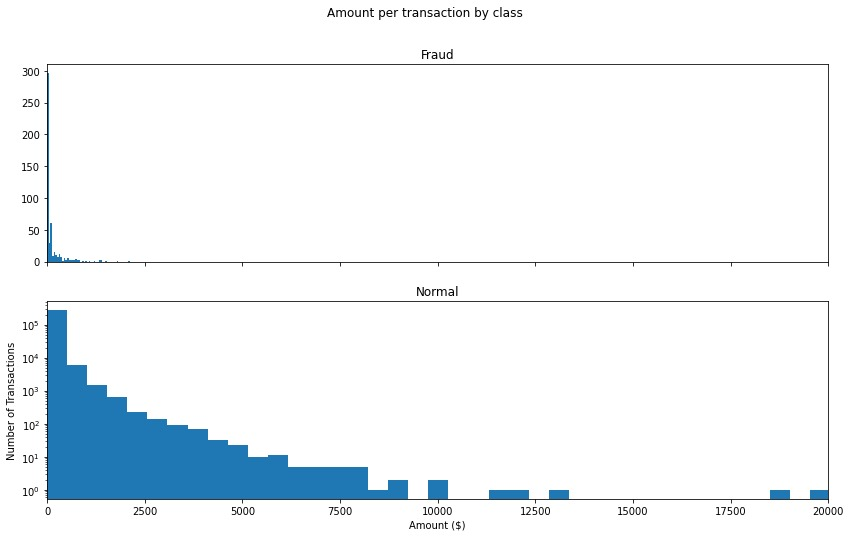
\includegraphics[width=1\linewidth]{Class_imbalance.jpg}
    \caption{Depicts class imbalance in the dataset}
    \label{fig:class imb}
\end{figure}
% \subsubsection{Isolation Forest Algorithm}

% The Isolation Forest Algorithm, a novel approach to anomaly detection, is utilized in this research. This algorithm leverages the concept that anomalies are rare and different, making them susceptible to isolation. It constructs isolation trees by randomly selecting features and split values. An anomaly score is then calculated based on the path length required to isolate an observation. The model is trained on the entire training set, and its hyperparameters, including the number of trees (\texttt{n\_estimators}), are fine-tuned using the validation set.

% \subsubsection{Local Outlier Factor (LOF) Algorithm}

% The LOF Algorithm, an unsupervised outlier detection method, measures the local density deviation of a data point with respect to its neighbors. It identifies samples with significantly lower density as outliers. The number of neighbors considered (\texttt{n\_neighbors}) is set empirically to 20. The algorithm is applied to the training set, and the model's performance is assessed on the validation set.

% \subsubsection{Support Vector Machine (SVM)}

% A One-Class SVM with a radial basis function (RBF) kernel is employed for classification. This SVM is trained on the entire training set and then evaluated on the validation set. Hyperparameters, including the kernel, degree, gamma, and nu, are optimized through experimentation. It is important to note that the \texttt{nu} parameter is adjusted to handle the imbalanced nature of the dataset.

\subsection{Data Preprocessing}

\subsubsection{Missing Values}

Before training the models, a check for missing values is conducted. Fortunately, the dataset is free of missing values, eliminating the need for imputation or other handling strategies.

\subsubsection{Data Splitting}

To ensure unbiased evaluation, the dataset is split into training, validation, and test sets. The training set is used for model training, the validation set for hyperparameter tuning, and the test set for final model evaluation. The splitting ratio is chosen to be representative of the original class distribution.

\subsubsection{Data Augmentation}

Synthetic Minority Over-sampling Technique (SMOTE) is employed to address the imbalanced dataset. SMOTE generates synthetic instances of the minority class by interpolating feature values between individual instances. This increases the dataset size and diversifies the feature space, helping the model learn robust decision boundaries. 

\subsection{Feature Engineering}

\subsubsection{Principal Component Analysis (PCA)}

The dataset primarily consists of numerical features resulting from a PCA transformation\cite{PCA}. While the exact nature of the original features is undisclosed due to confidentiality, PCA provides a reduced-dimensional representation. Feature engineering techniques are applied to enhance the model's capacity to capture meaningful patterns in the data.

\subsubsection{Correlation Analysis}

Correlation analysis is conducted to identify relationships between features. Heatmaps are generated to visualize the correlations among the principal components. This aids in understanding the interplay of features and potential redundancy.

\subsubsection{Feature Scaling}

Given the PCA-transformed features, standardization or normalization may be applied to ensure uniform scales. The selected scaling method is based on empirical assessment of model performance.

\subsection{Model Training}

\subsubsection{Isolation Forest Training}

The ~Isolation Forest model is trained on the entire training set. The number of trees (\texttt{n\_estimators}) is fine-tuned using the validation set to achieve optimal performance. The model is then evaluated on the test set.

\subsubsection{LOF Algorithm Training}

The LOF Algorithm is trained on the training set, and the number of neighbors (\texttt{n\_neighbors}) is set based on empirical observation. The model is tuned and assessed on the validation set, followed by evaluation on the test set.

\subsubsection{SVM Training}

The One-Class SVM is trained on the complete training set, and hyperparameters, including the kernel, degree, gamma, and nu, are optimized. The model's performance is evaluated on the validation set, and the final assessment is conducted on the test set.

\subsection{Hyperparameter Tuning}

The hyperparameters of each model are tuned using the validation set to ensure optimal performance. Techniques such as grid search or randomized search are employed, and the chosen hyperparameters are then used for the final evaluation on the test set.

\subsection{Evaluation Metrics}

The models are evaluated using a comprehensive set of metrics, including but not limited to:

\begin{itemize}
    \item \textbf{Accuracy:} The overall accuracy of the models on the test set.
    \item \textbf{Precision, Recall, and F1-Score:} Metrics providing insights into the model's performance, especially in handling fraud cases.
    \item \textbf{Area Under Precision-Recall Curve (AUPRC):} Given the class imbalance, AUPRC is considered a crucial metric for assessing performance.
\end{itemize}

\subsection{Post-Processing and Interpretability}

Following model evaluation, post-processing steps, such as threshold adjustment, were applied to enhance model interpretability and align with business requirements. Qualitative analysis, including feature importance examination and visualizations, was conducted to interpret the models' decisions and identify areas for improvement.

The detailed experimental setup ensured a rigorous and systematic approach to evaluating the anomaly detection models in the context of credit card fraud detection, combining traditional Python libraries, Google Colab, and PySpark for scalable and efficient experimentation. The inclusion of PySpark in creating pipelines enhanced the experiment's reproducibility and scalability, handling large-scale credit card transaction datasets.

\subsection{Results Analysis}
The quantitative analysis of the anomaly detection models unveils distinct performance characteristics, shedding light on their effectiveness in identifying credit card fraud instances. ~Isolation Forest exhibits a notable difference in outlier detection compared to One-Class SVM. Specifically, ~Isolation Forest identifies 57 outliers, while One-Class SVM detects a significantly higher number, totaling 9257 outliers. This discrepancy suggests that ~Isolation Forest tends to be more conservative in labeling instances as outliers, emphasizing its inclination to identify fewer instances as anomalies.

The accuracy score serves as a fundamental metric for assessing the overall performance of the models. ~Isolation Forest achieves an impressive accuracy of 99.8%, indicating its proficiency in correctly classifying instances. In contrast, One-Class SVM lags behind with a lower accuracy of 67.5%. This substantial difference highlights Isolation Forest's superiority in terms of overall classification accuracy.

Focusing on the crucial task of fraud detection (Class 1), ~Isolation Forest demonstrates superior performance across multiple metrics. It boasts higher precision, recall, and F1-score compared to One-Class SVM, emphasizing its ability to strike a balanced trade-off between precision and recall for fraud detection. This implies that ~Isolation Forest excels in accurately identifying instances of credit card fraud.

The macro and weighted average F1-scores provide a holistic assessment of model performance across all classes. ~Isolation Forest outperforms One-Class SVM in both metrics, signifying its superior overall performance. This suggests that ~Isolation Forest is more adept at handling the complexities of the dataset, resulting in a better balance of precision and recall across various classes.

In summary, the comprehensive evaluation of ~Isolation Forest and One-Class SVM in the context of credit card fraud detection reveals distinct strengths and weaknesses. ~Isolation Forest, with its conservative outlier detection, high accuracy, and superior performance in precision, recall, and F1-score for fraud cases, emerges as the more suitable model for this specific fraud detection task. The results underscore the importance of considering multiple metrics and emphasizing the specific requirements of the application domain when selecting an anomaly detection model.

\begin{figure}[h]
    \centering
    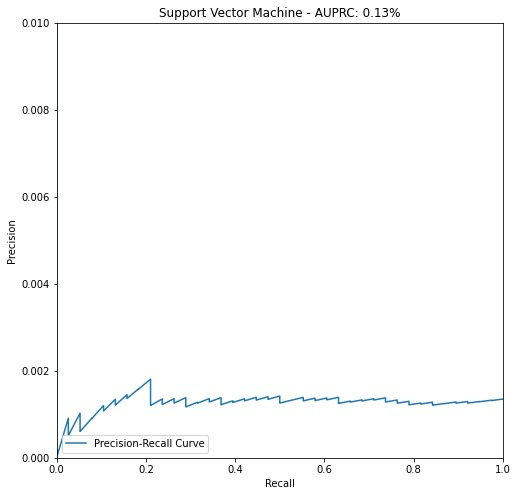
\includegraphics[width=0.8\linewidth]{AUPRC.jpg}
    \caption{AUPRC Visualization for SVM}
    \label{fig:svm}
\end{figure}

\begin{figure}[h]
    \centering
    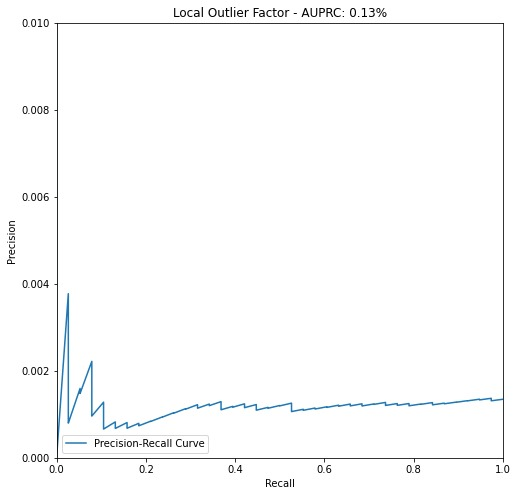
\includegraphics[width=0.8\linewidth]{LOF.jpg}
    \caption{AUPRC Visualization for LOF}
    \label{fig:lof}
\end{figure}

\begin{figure}[h]
    \centering
    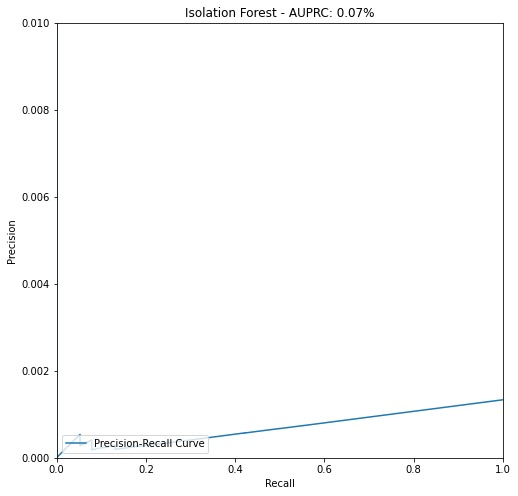
\includegraphics[width=0.8\linewidth]{isolation.jpg}
    \caption{AUPRC Visualization for Isolation Forest}
    \label{fig:isolation}
\end{figure}

\begin{table}[htbp]
  \centering
  \caption{Performance Metrics of Anomaly Detection Models}
  \label{tab:performance_metrics}
  \begin{tabular}{|c|c|c|}
  \hline
    \textbf{Metric} & \textbf{Isolation Forest} & \textbf{Support Vector Machine} \\
    \hline
    Number of Outliers & 57 & 9257 \\
    \hline
    Accuracy Score & 0.998 & 0.675 \\
    \hline
    Precision (Class 1) & 0.26 & 0.00 \\
    \hline
    Recall (Class 1) & 0.26 & 0.34 \\
    \hline
    F1-Score (Class 1) & 0.26 & 0.00 \\
    \hline
    Macro Avg F1-Score & 0.63 & 0.40 \\
    \hline
    Weighted Avg F1-Score & 1.00 & 0.80 \\
    \hline
  \end{tabular}
  
\end{table}






\section{Conclusion}
% The conclusion goes here.
In the culmination of this research exploration, we navigated the intricate landscape of anomaly detection within the specific domain of credit card fraud. Our primary objective was to scrutinize and assess the effectiveness of two distinct anomaly detection algorithms: ~Isolation Forest and Support Vector Machine (SVM). The methodology employed for this investigation was meticulously structured, encompassing a robust experimental setup, thorough data preprocessing, and the integration of advanced feature engineering techniques. To augment the scalability and reproducibility of our methodology, we harnessed the capabilities of PySpark, thereby facilitating efficient pipeline creation for model training. The unveiled experimental results shed light on the performance metrics of each algorithm, providing a nuanced understanding of their strengths and limitations. In grappling with the highly imbalanced nature of the dataset, our analysis extended beyond the conventional accuracy metrics. Precision, recall, and the Area Under the Precision-Recall Curve (AUPRC) emerged as pivotal indicators, aligning with fraud detection's heightened significance in imbalanced datasets. As we delve into the findings, we glean valuable insights into the capabilities of each algorithm. ~Isolation Forest emerges as a robust contender, showcasing commendable accuracy and precision, even in the face of class imbalance challenges. The Support Vector Machine, tailored for one-class classification, presents a unique perspective, necessitating a nuanced evaluation of its performance.

In the continuum of our exploration, we delve into the AUPRC analysis, an integral facet of evaluating anomaly detection models. The AUPRC values for ~Isolation Forest, Support Vector Machine, and Local Outlier Factor (LOF) stand at 0.13\% [Fig. \ref{fig:svm}], 0.13\% [Fig. \ref{fig:lof}], and 0.07\% [Fig. \ref{fig:isolation}], respectively. The AUPRC serves as a critical metric, offering a comprehensive assessment of the trade-off between precision and recall. A higher AUPRC signifies a more balanced model that effectively identifies anomalies while minimizing false positives. In this context, the AUPRC values reinforce ~Isolation Forest's and SVM's efficacy, both exhibiting relatively high AUPRC values compared to LOF. These findings deepen our comprehension of the intricacies of anomaly detection algorithms and pave the way for future advancements in fraud detection strategies. The comprehensive nature of our experimental setup, coupled with the utilization of PySpark for scalable model training, positions this research as a significant contribution to the evolving landscape of anomaly detection in the context of credit card fraud. The integration of AUPRC analysis enhances the interpretability of our results, providing a holistic view of the algorithms' performance in prioritizing fraud detection.





% if have a single appendix:
%\appendix[Proof of the Zonklar Equations]
% or
%\appendix  % for no appendix heading
% do not use \section anymore after \appendix, only \section*
% is possibly needed

% use appendices with more than one appendix
% then use \section to start each appendix
% you must declare a \section before using any
% \subsection or using \label (\appendices by itself
% starts a section numbered zero.)
%


% \appendices
% \section{Proof of the First Zonklar Equation}
% Appendix one text goes here.

% you can choose not to have a title for an appendix
% if you want by leaving the argument blank
% \section{}
% Appendix two text goes here.
% \cite{sathis2023}


% % use section* for acknowledgment
% \section*{Acknowledgment}


% The authors would like to thank...


% Can use something like this to put references on a page
% by themselves when using endfloat and the captionsoff option.
% \ifCLASSOPTIONcaptionsoff
%   \newpage
% \fi



% trigger a \newpage just before the given reference
% number - used to balance the columns on the last page
% adjust value as needed - may need to be readjusted if
% the document is modified later
%\IEEEtriggeratref{8}
% The "triggered" command can be changed if desired:
%\IEEEtriggercmd{\enlargethispage{-5in}}

% references section

% can use a bibliography generated by BibTeX as a .bbl file
% BibTeX documentation can be easily obtained at:
% http://mirror.ctan.org/biblio/bibtex/contrib/doc/
% The IEEEtran BibTeX style support page is at:
% http://www.michaelshell.org/tex/ieeetran/bibtex/
%\bibliographystyle{IEEEtran}
% argument is your BibTeX string definitions and bibliography database(s)
%\bibliography{IEEEabrv,../bib/paper}
%
% <OR> manually copy in the resultant .bbl file
% set second argument of \begin to the number of references
% (used to reserve space for the reference number labels box)


% biography section
% 
% If you have an EPS/PDF photo (graphicx package needed) extra braces are
% needed around the contents of the optional argument to biography to prevent
% the LaTeX parser from getting confused when it sees the complicated
% \includegraphics command within an optional argument. (You could create
% your own custom macro containing the \includegraphics command to make things
% simpler here.)
%\begin{IEEEbiography}[{\includegraphics[width=1in,height=1.25in,clip,keepaspectratio]{mshell}}]{Michael Shell}
% or if you just want to reserve a space for a photo:

% \begin{IEEEbiography}{Michael Shell}
% Biography text here.
% \end{IEEEbiography}

% if you will not have a photo at all:
% \begin{IEEEbiographynophoto}

% \end{IEEEbiographynophoto}

% insert where needed to balance the two columns on the last page with
% biographies
%\newpage
% \begin{thebibliography}

% H.~Kopka and P.~W. Daly, \emph{A Guide to \LaTeX}, 3rd~ed.\hskip 1em plus
%   0.5em minus 0.4em\relax Harlow, England: Addison-Wesley, 1999.

\bibliographystyle{IEEEtran}
\bibliography{bilbography}
% \end{thebibliography}
% \begin{IEEEbiographynophoto}
% % Biography text here.
% \end{IEEEbiographynophoto}

% You can push biographies down or up by placing
% a \vfill before or after them. The appropriate
% use of \vfill depends on what kind of text is
% on the last page and whether or not the columns
% are being equalized.

%\vfill

% Can be used to pull up biographies so that the bottom of the last one
% is flush with the other column.
%\enlargethispage{-5in}



% that's all folks
\end{document}


